\documentclass[11pt]{article}

\usepackage{graphicx}
\usepackage{amsmath}
\usepackage[utf8]{inputenc}
\usepackage[T1]{fontenc}
\usepackage[lithuanian]{babel}
\usepackage{listings}
\lstset{
    inputencoding=utf8,
    extendedchars=false
}

\usepackage[
    a4paper,
    bindingoffset=0.2in,
    left=1in,
    right=1in,
    top=1in,
    bottom=1in,
    footskip=.25in]{geometry}

\title{ Trečias laboratorinis darbas}
\author{ Arnas Vaicekauskas }
\date{\today}

\begin{document}

\maketitle

\section{Analitinis sprendimas}
Turime antros eilės tiesinę nehomogeninę lygtį su pradinėmis sąlygomis:
\begin{align}
x''+9x&=4\sin(t)-\cos(4t) \label{eqs:nohom}\\
x(0)&=0\label{eqs:initial-1}\\
x'(0)&=1\label{eqs:initial-2}
\end{align}
Pirmiausia spręsime homogeninį atvejį norint gauti bendrąjį sprendinį:
\begin{align}
    x''+9x=0 \label{eqs:hom}
\end{align}
Lygtis \eqref{eqs:hom} turi pastovius koeficientus, 
todėl galime formuoti charakteringąjį polinomą
\begin{align*}
    \lambda^2+9=0\implies\lambda=\pm3i
\end{align*}
Šiuo atveju bendrasis sprendinys $x_B(t)$ turės formą 
\begin{align*}
x_B(t)=C_1e^{3it}+C_2e^{-3it}
\end{align*}
Nehomogeninę lygtį \eqref{eqs:nohom} spręsime
konstantų variavimo metodu, todėl:
\begin{align}
x(t)=C_1(t)e^{3it}+C_2(t)e^{-3it} \label{eqs:varsol}
\end{align}
Pagal variavimo metodą, darome prielaidą, kad 
\begin{align}
C_1'e^{3it}+C_2'e^{-3it}=0  \label{eqs:assumtion}
\end{align}
Prieš įstatant varijuotą bendrąjį sprendinį \eqref{eqs:varsol} apskaičiuosime $x''$ ir $x''+9x$: 
\begin{align*}
x''&=(C_1'e^{3it}+3iC_1e^{3it}+C_2'e^{-3it}-3iC_2e^{-3it})'\\
&=(\underbrace{C_1'e^{3it}+C_2'e^{-3it}}_0+3iC_1e^{3it}-3iC_2e^{-3it})'\\
&=(3iC_1e^{3it}-3iC_2e^{-3it})'\\
&=3iC_1'e^{3it}-9C_1e^{3it}-3iC_2'e^{-3it}-9C_2e^{-3it}
\end{align*}
Tada
\begin{align*}
x''+9x&=3iC_1'e^{3it}-9C_1e^{3it}-3iC_2'e^{-3it}-9C_2e^{-3it}+9C_1e^{3it}+9C_2e^{-3it}\\
&=3iC_1'e^{3it}-3iC_2'e^{-3it}
\end{align*}
Taigi, dabar sprendžiame lygtį
\begin{align}
3iC_1'e^{3it}-3iC_2'e^{-3it}=4\sin(t)-\cos(4t)\label{eqs:variated}
\end{align}
Naudodami tapatybes $\sin(t)=\frac{e^{it}-e^{-it}}{2i}$, $\cos(t)=\frac{e^{it}+e^{-it}}{2}$, $\frac{1}{i}=-i$ galime pertvarkyti lygtį \eqref{eqs:variated}
\begin{align}
3iC_1'e^{3it}-3iC_2'e^{-3it}&=4\frac{e^{it}-e^{-it}}{2i}-\frac{e^{4it}+e^{-4it}}{2}\notag\\
3iC_1'e^{3it}-3iC_2'e^{-3it}&=\frac{2e^{it}}{i}-\frac{2e^{-it}}{i}-\frac{e^{4it}}{2}-\frac{e^{-4it}}{2}\notag\\
3iC_1'e^{3it}-3iC_2'e^{-3it}&=-2ie^{it}+2ie^{-it}-\frac{e^{4it}}{2}-\frac{e^{-4it}}{2}\label{eqs:1}
\end{align}
Iš prielaidos \eqref{eqs:assumtion} galime išsireikšti $C_2'$
\begin{align}
C_2'=-C_1'e^{6it} \label{eqs:c1c2}    
\end{align}
Tuomet įstatome lygties \eqref{eqs:c1c2} dešinę pusę į lygtį \eqref{eqs:1}
\begin{align}
3iC_1'e^{3it}+3iC_1'e^{6it}e^{-3it}&=-2ie^{it}+2ie^{-it}-\frac{e^{4it}}{2}-\frac{e^{-4it}}{2} \notag\\
6iC_1'e^{3it}&=-2ie^{it}+2ie^{-it}-\frac{e^{4it}}{2}-\frac{e^{-4it}}{2} \notag\\
C_1'&=\frac{e^{-3it}}{6i}\left(-2ie^{it}+2ie^{-it}-\frac{e^{4it}}{2}-\frac{e^{-4it}}{2}\right) \notag\\
C_1'&=-\frac{e^{-2it}}{3}+\frac{e^{-4it}}{3}-\frac{e^{it}}{12i}-\frac{e^{-7it}}{12i} \label{eqs:c1d}\\
C_1&=\int\left(-\frac{e^{-2it}}{3}+\frac{e^{-4it}}{3}-\frac{e^{it}}{12i}-\frac{e^{-7it}}{12i}\right)dt \notag\\
C_1&=-\frac{1}{-2i}\frac{e^{-2it}}{3}+\frac{1}{-4i}\frac{e^{-4it}}{3}-\frac{1}{i}\frac{e^{it}}{12i}-\frac{1}{-7i}\frac{e^{-7it}}{12i}+\tilde{C_1}\notag\\
C_1(t)&=\frac{e^{-2it}}{6i}-\frac{e^{-4it}}{12i}+\frac{e^{it}}{12}-\frac{e^{-7it}}{84}+\tilde{C_1} \label{eqs:c1}
\end{align}
Į lygtį \eqref{eqs:c1c2} įstate \eqref{eqs:c1d} gauname $C_2'$ ir integrave gauname $C_2$:
\begin{align}
C_2'&=-e^{6it}C_1'\notag\\
C_2'&=-e^{6it}\left(-\frac{e^{-2it}}{3}+\frac{e^{-4it}}{3}-\frac{e^{it}}{12i}-\frac{e^{-7it}}{12i}\right)\notag\\
C_2'&=\frac{e^{4it}}{3}-\frac{e^{2it}}{3}+\frac{e^{7it}}{12i}+\frac{e^{-it}}{12i}\notag\\
C_2&=\int\left(\frac{e^{4it}}{3}-\frac{e^{2it}}{3}+\frac{e^{7it}}{12i}+\frac{e^{-it}}{12i}\right)dt\notag\\
C_2&=\frac{1}{4i}\frac{e^{4it}}{3}-\frac{1}{2i}\frac{e^{2it}}{3}+\frac{1}{7i}\frac{e^{7it}}{12i}+\frac{1}{-i}\frac{e^{-it}}{12i}+\tilde{C_2}\notag\\
C_2&=\frac{e^{4it}}{12i}-\frac{e^{2it}}{6i}-\frac{e^{7it}}{84}+\frac{e^{-it}}{12}+\tilde{C_2}\label{eqs:c2}
\end{align}
Įstačius gautas $C_1$ ir $C_2$ išraiškas \eqref{eqs:c1} ir \eqref{eqs:c2} gauname nehomogeninės lygties sprendinį:
\begin{align}
x(t)&=\left(\frac{e^{-2it}}{6i}-\frac{e^{-4it}}{12i}+\frac{e^{it}}{12}-\frac{e^{-7it}}{84}+\tilde{C_1}\right)e^{3it}
+\left(\frac{e^{4it}}{12i}-\frac{e^{2it}}{6i}-\frac{e^{7it}}{84}+\frac{e^{-it}}{12}+\tilde{C_2}\right)e^{-3it}\notag\\
x(t)&=\frac{e^{it}}{6i}-\frac{e^{-it}}{12i}+\frac{e^{4it}}{12}-\frac{e^{-4it}}{84}+\tilde{C_1}e^{3it}
+\frac{e^{it}}{12i}-\frac{e^{-it}}{6i}-\frac{e^{4it}}{84}+\frac{e^{-4it}}{12}+\tilde{C_2}e^{-3it}\notag\\
x(t)&=\frac{1}{2}\frac{e^{it}-e^{-it}}{2i}+\frac{1}{7}\frac{e^{4it}+e^{-4it}}{2}+\tilde{C_1}\frac{e^{3it}-e^{-3it}}{2i}+\tilde{C_2}\frac{e^{3it}+e^{-3it}}{2}\notag\\
x(t)&=\frac{\sin(t)}{2}+\frac{\cos(4t)}{7}+\tilde{C_1}\sin(3t)+\tilde{C_2}\cos(3t)\label{eqs:gen-sol}
\end{align}
Randame Koši sprendinį įstatant pradines sąlygas \eqref{eqs:initial-1} ir \eqref{eqs:initial-2} į lygtį \eqref{eqs:gen-sol}:
\begin{align*}
x(0)=0\\
\frac{0}{2}+\frac{\cos(0)}{7}+\tilde{C_1}\sin(0)+\tilde{C_2}\cos(0)=0\\
\frac{1}{7}+\tilde{C_2}=0\\
\tilde{C_2}=-\frac{1}{7}\\
x'(0)=1\\
\left(\frac{\sin(t)}{2}+\frac{\cos(4t)}{7}+\tilde{C_1}\sin(3t)-\frac{1}{7}\cos(3t)\right)'\Big\vert_{x=0}=1\\
\left(-\frac{\cos(t)}{2}-4\frac{\sin(4t)}{7}+3\tilde{C_1}\cos(3t)+\frac{3}{7}\sin(3t)\right)\Big\vert_{x=0}=1\\
\frac{\cos(0)}{2}-4\frac{\sin(0)}{7}+3\tilde{C_1}\cos(0)+\frac{3}{7}\sin(0)=1\\
\frac{1}{2}+3\tilde{C_1}=1\\
\tilde{C_1}=\frac{1}{6}\\
\end{align*}
Koši sprendinys:
\begin{align}
x(t)&=\frac{\sin(t)}{2}+\frac{\cos(4t)}{7}+\frac{\sin(3t)}{6}-\frac{\cos(3t)}{7}\label{eqs:cauchy-sol}
\end{align} 
Kai $t\to+\infty$ sprendinys $x(t)$ nekonverguoja, nes trigonometrinių funkcijų svyravimas 
nėra slopinamas, t.y. riba neegzistuoja.
$$\lim_{t\to+\infty}x(t)=DNE$$
Koši sprendinio svyravimų periodą galima rasti pažvelgus į individualiu sprendinio dėmenų svyravimo periodus.
\begin{align*}
\sin(t)\implies T=\frac{2\pi}{1}=2\pi\\
\sin(3t)\implies T=\frac{2\pi}{3}\\
\cos(3t)\implies T=\frac{2\pi}{3}\\
\cos(4t)\implies T=\frac{2\pi}{4}=\frac{\pi}{2}
\end{align*}
Individualių sprendinio dėmenų svyravimų periodų mažiausias bendras kartotinis yra $2\pi$, todėl ir $x(t)$ svyravimo periodas yra $T=2\pi$. Analitinis sprendinio amplitudės radimas yra
už šio darbo apimties, todėl pateiktos reikšmės buvo rastos naudojant skaitinius metodus.
\begin{align*}
\min_{t\in[0,2\pi]}x(t)&\approx -0.7252871753033927\\
\max_{t\in[0,2\pi]}x(t)&\approx 0.537908854609837
\end{align*}
\section{Palyginimas su programos sprendiniu}
Programa rasti lygties \eqref{eqs:nohom} sprendiniui su pradinėmis sąlygomis \eqref{eqs:initial-1} bei \eqref{eqs:initial-2} buvo rašyta su python programavimo
kalba bei sympy paketu. Programa rastas sprendinys
\begin{align}
x(t)=\frac{\sin(t)}{2}+\frac{\sin(3t)}{6}-\frac{\cos(3t)}{7}+\frac{\cos(4t)}{7}\label{eqs:program-sol}
\end{align}
Yra akivaizdu, kad analitiškai \eqref{eqs:cauchy-sol} ir programa \eqref{eqs:program-sol} gauti sprendiniai yra ekvivalentūs.
\section{Sprendinio grafikas}
\begin{figure}[h!]
\centering
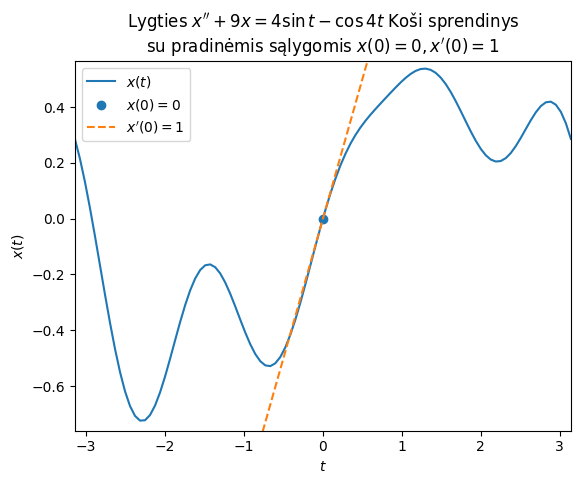
\includegraphics[width=0.5\textwidth]{graph.png}
\caption{Lygties \eqref{eqs:nohom} Koši sprendinys}
\label{fig:cauchy-sol}
\end{figure}
\section{Priedai}
Kodas naudotas rasti lygties \eqref{eqs:nohom} Koši sprendinį su pradinėmis sąlygomis \eqref{eqs:initial-1} ir \eqref{eqs:initial-2}
\begin{lstlisting}[language=Python]
from sympy import *
t = symbols('t')
x = Function('x')(t)
equation = Eq(x.diff(t, 2) + 9*x, 4 * sin(t) - cos(4 * t))
general_solution = dsolve(equation, x).rhs
conditions = [
    Eq(general_solution.subs(t, 0), 0),
    Eq(general_solution.diff(t).subs(t, 0), 1)
]
C_values = solve(conditions, symbols("C1, C2"))
general_solution.subs(C_values)
\end{lstlisting}
\newpage
Kodas naudotas pavaizduoti Koši sprendinį \eqref{eqs:cauchy-sol}
\begin{lstlisting}[language=Python]
import numpy as np
import matplotlib.pyplot as plt
def x(t):
    return np.sin(t)/2 + np.cos(4*t)/7+np.sin(3*t)/6-np.cos(3*t)/7
ts = np.linspace(0, 2 * np.pi, 100)
title ="""Lygties $x''+9x=4\sin t-\cos 4t$ Koši sprendinys
su pradinėmis sąlygomis $x(0)=0, x'(0)=1$"""
plt.title(title)
plt.plot(ts, x(ts), label='x(t)')
plt.xlabel('$t$')
plt.ylabel('$x(t)$')
plt.legend()
\end{lstlisting}
Kodas naudotas rasti Koši sprendinio \eqref{eqs:cauchy-sol} svyravimo amplitudę
\begin{lstlisting}[language=Python]
import numpy as np
def x(t):
    return np.sin(t)/2 + np.cos(4*t)/7+np.sin(3*t)/6-np.cos(3*t)/7
ts = np.linspace(0, 2 * np.pi, 1000)
xs = x(ts)
np.min(xs), np.max(xs)
\end{lstlisting}
\end{document}

